\documentclass[border=3pt,tikz]{standalone}
\usepackage{amsmath}
\usetikzlibrary {arrows.meta}
\usetikzlibrary {calc}
\begin{document}
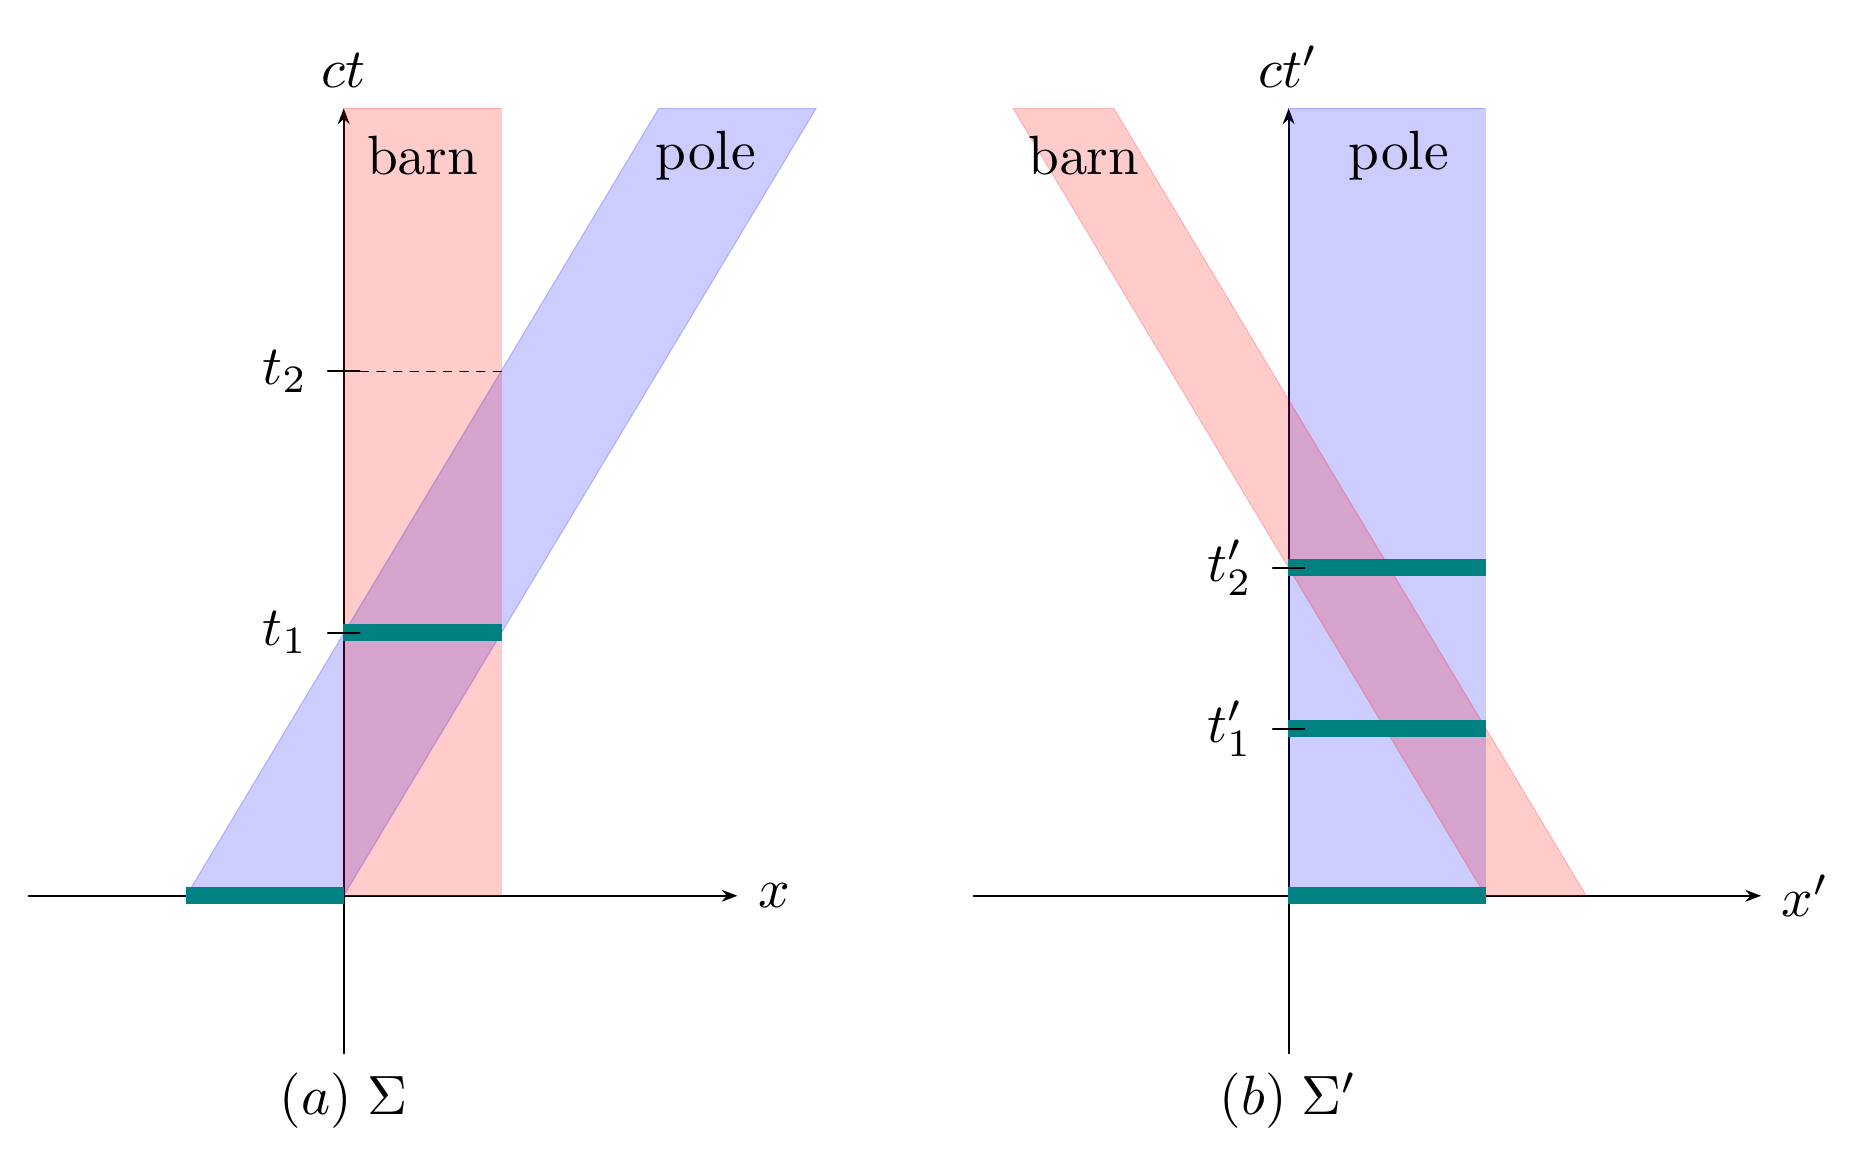
\begin{tikzpicture}[line cap=round, scale = 2]

    % font scale
    \def\fs{2.0}
    \def\tk{0.05}
    
    \draw [thick, -{Stealth[length=2mm]}] (-2., 0) -- (2.5, 0) node [right, scale=\fs] {$x$};
    \draw [thick, -{Stealth[length=2mm]}] (0, -1) -- (0, 5) node [above, scale=\fs] {$ct$};
    
    \filldraw [blue, opacity=0.2] (-1.0, 0) -- (2, 5) -- (3.0, 5) -- (-0.0, 0) -- cycle;
    \filldraw [red, opacity=0.2] (0, 0) -- (0, 5) -- (1, 5) -- (1, 0) -- cycle;
    \node[scale=\fs] at (0.5, 4.7) {$\textrm{barn}$};
    \node[scale=\fs] at (2.3, 4.7) {$\textrm{pole}$};
    
    \filldraw[teal] (-1.0, \tk) -- (-0.0, \tk) -- (-0.0, -\tk) -- (-1.0, -\tk) --cycle; 
    \filldraw[teal] (0, 1.67 + \tk) -- (1, 1.67 +\tk) -- (1, 1.67-\tk) -- (0, 1.67-\tk) --cycle; 
    
    \draw[thick] (-0.1, 1.67) node[left, scale=\fs] {$t_1$}-- (0.1, 1.67);
    \draw[thick] (-0.1, 3.33) node[left, scale=\fs] {$t_2$}-- (0.1, 3.33);
    \draw[dashed] (0.0, 3.33) -- (1.0, 3.33);
    
    \node[below, scale=\fs] at(0, -1) {$(a)\;\Sigma$};
    
    
    \begin{scope}[xshift=6cm]
    
    \draw [thick, -{Stealth[length=2mm]}] (-2., 0) -- (3, 0) node [right, scale=\fs] {$x'$};
    \draw [thick, -{Stealth[length=2mm]}] (0, -1) -- (0, 5) node [above, scale=\fs] {$ct'$};
    
    \filldraw [blue, opacity=0.2] (0.0, 0) -- (0, 5) -- (1.25, 5) -- (1.25, 0) -- cycle;
    \filldraw [red, opacity=0.2] (1.25, 0) -- (-1.75, 5) -- (-1.11, 5) -- (1.89, 0) -- cycle;
    \node[scale=\fs] at (-1.3, 4.7) {$\textrm{barn}$};
    \node[scale=\fs] at (0.7, 4.7) {$\textrm{pole}$};
    
    \filldraw[teal] (0, \tk) -- (1.25, \tk) -- (1.25, -\tk) -- (0, -\tk) --cycle; 
    \filldraw[teal] (0, 2.083 + \tk) -- (1.25, 2.083+\tk) -- (1.25, 2.083-\tk) -- (0, 2.083-\tk) --cycle; 
    \filldraw[teal] (0, 1.06 + \tk) -- (1.25, 1.06+\tk) -- (1.25, 1.06-\tk) -- (0, 1.06-\tk) --cycle; 
    
    
    \draw[thick] (-0.1, 1.06) node[left, scale=\fs] {$t_1'$}-- (0.1, 1.06);
    \draw[thick] (-0.1, 2.083) node[left, scale=\fs] {$t_2'$}-- (0.1, 2.083);
    
    \node[below, scale=\fs] at(0, -1) {$(b)\;\Sigma'$};
    \end{scope}
    \end{tikzpicture}

\end{document}